Consider the positive-feedback circuit shown in Fig. \ref{fig:ee18btech11030}. 
\begin{figure}[!ht]
	\begin{center}
		\resizebox{\columnwidth/1}{!}{ 
\usetikzlibrary{decorations.markings}
\begin{circuitikz}
\draw (-4,-1) to[amp,t={+K}] (2.5,-1);
\draw (-4,-1) to (-4,2) to (-3,2) ;
\draw (-3,2)  to [capacitor=$C/10$](-3,0.5) to  (-3,0.5) node[ground]{};
\draw (-3,2) to (-2.3,2)to [R=$10R$] (-1.3,2)to (0,2) to [R=$R$] (0,5) node[label={}]{}  to (-4,5) ;
\draw (0,2) to(1,2) to  [capacitor=$C$](1.5,2) to (2.5,2) to (2.5,-1);
\draw (-4,5) to (-4,4.7) to [V=$V_s$] (-4,3.9) to (-4,3.5) node[ground]{} ;
\draw (2.5,-1) to[short, -o] (3,-1) node[label={above:$V_{out}$}]{};
\end{circuitikz}}
	\end{center}
	\caption{ Positive Feedback Circuit}
	\label{fig:ee18btech11030}
\end{figure}
\begin{enumerate}[label=(\alph*),ref=\theenumi]

\item Find the loop transmission L(s) and the characteristic equation ,find the expressions for resulting pole frequency $\omega_o$ and Q factor?
\item Sketch a Pole-Zero plot for varying K. 
\item For what value of K do the poles coincide? For what value of K does the response becomes maximally flat? For what value of K does the circuit oscillate?
\end{enumerate}
Assume that the amplifier has frequency-independent gain, infinite input impedance, and zero output impedance.
%\begin{enumerate}[label=\thesubsection.\arabic*.,ref=\thesubsection.\theenumi]
\begin{enumerate}[label=\arabic*.,ref=\theenumi]
\numberwithin{equation}{enumi}
\item Find $L(s)$.

\solution To obtain the loop transmission L(s),
\begin{itemize}
\item Short-circuit the signal source $V_s$.
\item Break the loop at the Amplifier input.
\item Then apply a test voltage $V_t$ and find the returned voltage $V_r$, as indicated in Figure: \ref{fig:ee18btech11030_fig1}.
\end{itemize}

\begin{figure}[!ht]
	\begin{center}
		\resizebox{\columnwidth/1}{!}{%%%%%%%%%%%%%%%%%%%%%%%%%%%%%%%%%%%%%%%%%%%%%%%%%%%%%%%%%%%%%%%%%%%%%%
%%                                                                  %%
%%  This is the header of a LaTeX2e file exported from Gnumeric.    %%
%%                                                                  %%
%%  This file can be compiled as it stands or included in another   %%
%%  LaTeX document. The table is based on the longtable package so  %%
%%  the longtable options (headers, footers...) can be set in the   %%
%%  preamble section below (see PRAMBLE).                           %%
%%                                                                  %%
%%  To include the file in another, the following two lines must be %%
%%  in the including file:                                          %%
%%        \def\inputGnumericTable{}                                 %%
%%  at the beginning of the file and:                               %%
%%        \input{name-of-this-file.tex}                             %%
%%  where the table is to be placed. Note also that the including   %%
%%  file must use the following packages for the table to be        %%
%%  rendered correctly:                                             %%
%%    \usepackage[latin1]{inputenc}                                 %%
%%    \usepackage{color}                                            %%
%%    \usepackage{array}                                            %%
%%    \usepackage{longtable}                                        %%
%%    \usepackage{calc}                                             %%
%%    \usepackage{multirow}                                         %%
%%    \usepackage{hhline}                                           %%
%%    \usepackage{ifthen}                                           %%
%%  optionally (for landscape tables embedded in another document): %%
%%    \usepackage{lscape}                                           %%
%%                                                                  %%
%%%%%%%%%%%%%%%%%%%%%%%%%%%%%%%%%%%%%%%%%%%%%%%%%%%%%%%%%%%%%%%%%%%%%%



%%  This section checks if we are begin input into another file or  %%
%%  the file will be compiled alone. First use a macro taken from   %%
%%  the TeXbook ex 7.7 (suggestion of Han-Wen Nienhuys).            %%
\def\ifundefined#1{\expandafter\ifx\csname#1\endcsname\relax}


%%  Check for the \def token for inputed files. If it is not        %%
%%  defined, the file will be processed as a standalone and the     %%
%%  preamble will be used.                                          %%
\ifundefined{inputGnumericTable}

%%  We must be able to close or not the document at the end.        %%
	\def\gnumericTableEnd{\end{document}}


%%%%%%%%%%%%%%%%%%%%%%%%%%%%%%%%%%%%%%%%%%%%%%%%%%%%%%%%%%%%%%%%%%%%%%
%%                                                                  %%
%%  This is the PREAMBLE. Change these values to get the right      %%
%%  paper size and other niceties.                                  %%
%%                                                                  %%
%%%%%%%%%%%%%%%%%%%%%%%%%%%%%%%%%%%%%%%%%%%%%%%%%%%%%%%%%%%%%%%%%%%%%%

	\documentclass[12pt%
			  %,landscape%
                    ]{report}
       \usepackage[latin1]{inputenc}
       \usepackage{fullpage}
       \usepackage{color}
       \usepackage{array}
       \usepackage{longtable}
       \usepackage{calc}
       \usepackage{multirow}
       \usepackage{hhline}
       \usepackage{ifthen}



%%  End of the preamble for the standalone. The next section is for %%
%%  documents which are included into other LaTeX2e files.          %%
\else

%%  We are not a stand alone document. For a regular table, we will %%
%%  have no preamble and only define the closing to mean nothing.   %%
    \def\gnumericTableEnd{}

%%  If we want landscape mode in an embedded document, comment out  %%
%%  the line above and uncomment the two below. The table will      %%
%%  begin on a new page and run in landscape mode.                  %%
%       \def\gnumericTableEnd{\end{landscape}}
%       \begin{landscape}


%%  End of the else clause for this file being \input.              %%
\fi

%%%%%%%%%%%%%%%%%%%%%%%%%%%%%%%%%%%%%%%%%%%%%%%%%%%%%%%%%%%%%%%%%%%%%%
%%                                                                  %%
%%  The rest is the gnumeric table, except for the closing          %%
%%  statement. Changes below will alter the table's appearance.     %%
%%                                                                  %%
%%%%%%%%%%%%%%%%%%%%%%%%%%%%%%%%%%%%%%%%%%%%%%%%%%%%%%%%%%%%%%%%%%%%%%

\providecommand{\gnumericmathit}[1]{#1} 
%%  Uncomment the next line if you would like your numbers to be in %%
%%  italics if they are italizised in the gnumeric table.           %%
%\renewcommand{\gnumericmathit}[1]{\mathit{#1}}
\providecommand{\gnumericPB}[1]%
{\let\gnumericTemp=\\#1\let\\=\gnumericTemp\hspace{0pt}}
 \ifundefined{gnumericTableWidthDefined}
        \newlength{\gnumericTableWidth}
        \newlength{\gnumericTableWidthComplete}
        \newlength{\gnumericMultiRowLength}
        \global\def\gnumericTableWidthDefined{}
 \fi
%% The following setting protects this code from babel shorthands.  %%
 \ifthenelse{\isundefined{\languageshorthands}}{}{\languageshorthands{english}}
%%  The default table format retains the relative column widths of  %%
%%  gnumeric. They can easily be changed to c, r or l. In that case %%
%%  you may want to comment out the next line and uncomment the one %%
%%  thereafter                                                      %%
\providecommand\gnumbox{\makebox[0pt]}
%%\providecommand\gnumbox[1][]{\makebox}

%% to adjust positions in multirow situations                       %%
\setlength{\bigstrutjot}{\jot}
\setlength{\extrarowheight}{\doublerulesep}

%%  The \setlongtables command keeps column widths the same across  %%
%%  pages. Simply comment out next line for varying column widths.  %%
\setlongtables

\setlength\gnumericTableWidth{%
	50pt+%
	65pt+%
0pt}
\def\gumericNumCols{2}
\setlength\gnumericTableWidthComplete{\gnumericTableWidth+%
         \tabcolsep*\gumericNumCols*2+\arrayrulewidth*\gumericNumCols}
\ifthenelse{\lengthtest{\gnumericTableWidthComplete > \linewidth}}%
         {\def\gnumericScale{\ratio{\linewidth-%
                        \tabcolsep*\gumericNumCols*2-%
                        \arrayrulewidth*\gumericNumCols}%
{\gnumericTableWidth}}}%
{\def\gnumericScale{1}}

%%%%%%%%%%%%%%%%%%%%%%%%%%%%%%%%%%%%%%%%%%%%%%%%%%%%%%%%%%%%%%%%%%%%%%
%%                                                                  %%
%% The following are the widths of the various columns. We are      %%
%% defining them here because then they are easier to change.       %%
%% Depending on the cell formats we may use them more than once.    %%
%%                                                                  %%
%%%%%%%%%%%%%%%%%%%%%%%%%%%%%%%%%%%%%%%%%%%%%%%%%%%%%%%%%%%%%%%%%%%%%%

\ifthenelse{\isundefined{\gnumericColA}}{\newlength{\gnumericColA}}{}\settowidth{\gnumericColA}{\begin{tabular}{@{}p{53pt*\gnumericScale}@{}}x\end{tabular}}
\ifthenelse{\isundefined{\gnumericColB}}{\newlength{\gnumericColB}}{}\settowidth{\gnumericColB}{\begin{tabular}{@{}p{93pt*\gnumericScale}@{}}x\end{tabular}}

\begin{tabular}[c]{%
	b{\gnumericColA}%
	b{\gnumericColB}%
	}

%%%%%%%%%%%%%%%%%%%%%%%%%%%%%%%%%%%%%%%%%%%%%%%%%%%%%%%%%%%%%%%%%%%%%%
%%  The longtable options. (Caption, headers... see Goosens, p.124) %%
%	\caption{The Table Caption.}             \\	%
% \hline	% Across the top of the table.
%%  The rest of these options are table rows which are placed on    %%
%%  the first, last or every page. Use \multicolumn if you want.    %%

%%  Header for the first page.                                      %%
%	\multicolumn{2}{c}{The First Header} \\ \hline 
%	\multicolumn{1}{c}{colTag}	%Column 1
%	&\multicolumn{1}{c}{colTag}	\\ \hline %Last column
%	\endfirsthead

%%  The running header definition.                                  %%
%	\hline
%	\multicolumn{2}{l}{\ldots\small\slshape continued} \\ \hline
%	\multicolumn{1}{c}{colTag}	%Column 1
%	&\multicolumn{1}{c}{colTag}	\\ \hline %Last column
%	\endhead

%%  The running footer definition.                                  %%
%	\hline
%	\multicolumn{2}{r}{\small\slshape continued\ldots} \\
%	\endfoot

%%  The ending footer definition.                                   %%
%	\multicolumn{2}{c}{That's all folks} \\ \hline 
%	\endlastfoot
%%%%%%%%%%%%%%%%%%%%%%%%%%%%%%%%%%%%%%%%%%%%%%%%%%%%%%%%%%%%%%%%%%%%%%

\hhline{|-|-}
	 \multicolumn{1}{|p{\gnumericColA}|}%
	{\gnumericPB{\centering}\gnumbox{\textbf{Parameter}}}
	&\multicolumn{1}{p{\gnumericColB}|}%
	{\gnumericPB{\centering}\gnumbox{\textbf{Value}}}
\\
\hhline{|--|}
	 \multicolumn{1}{|p{\gnumericColA}|}%
	{\gnumericPB{\raggedright}\gnumbox[l]{$R_{1}$}}
	&\multicolumn{1}{p{\gnumericColB}|}%
	{\gnumericPB{\raggedright}\gnumbox[l]{$10k\Omega$}}
\\
\hhline{|--|}
	 \multicolumn{1}{|p{\gnumericColA}|}%
	{\gnumericPB{\raggedright}\gnumbox[l]{$R_{2}$}}
	&\multicolumn{1}{p{\gnumericColB}|}%
	{\gnumericPB{\raggedright}\gnumbox[l]{$11.3k\Omega$}}
\\
\hhline{|--|}
	 \multicolumn{1}{|p{\gnumericColA}|}%
	{\gnumericPB{\raggedright}\gnumbox[l]{$R$}}
	&\multicolumn{1}{p{\gnumericColB}|}%
	{\gnumericPB{\raggedright}\gnumbox[l]{$10k\Omega$}}
\\
\hhline{|--|}
	 \multicolumn{1}{|p{\gnumericColA}|}%
	{\gnumericPB{\raggedright}\gnumbox[l]{$10R$}}
	&\multicolumn{1}{p{\gnumericColB}|}%
	{\gnumericPB{\raggedright}\gnumbox[l]{$100k\Omega$}}
\\
\hhline{|--|}
	 \multicolumn{1}{|p{\gnumericColA}|}%
	{\gnumericPB{\raggedright}\gnumbox[l]{$C/10$}}
	&\multicolumn{1}{p{\gnumericColB}|}%
	{\gnumericPB{\raggedright}\gnumbox[l]{$1.6nF$}}
\\

\hhline{|--|}
	 \multicolumn{1}{|p{\gnumericColA}|}%
	{\gnumericPB{\raggedright}\gnumbox[l]{$C$}}
	&\multicolumn{1}{p{\gnumericColB}|}%
	{\gnumericPB{\raggedright}\gnumbox[l]{$16nF$}}

\\
\hhline{|-|-|}
\end{tabular}

\ifthenelse{\isundefined{\languageshorthands}}{}{\languageshorthands{\languagename}}
\gnumericTableEnd
}
	\end{center}
	\caption{}
	\label{fig:ee18btech11030_fig1}
\end{figure}

The loop transmission is given by
\begin{align}
    L\brak{s} = -\frac{V_r\brak{s}}{V_t\brak{s}} = -KT\brak{s}
\label{eq:ee18btech11030}
\end{align}
where T(s) is the transfer function of the two-port RC network shown inside the broken-line box in Figure: \ref{fig:ee18btech11030_fig1}.

\begin{align}
T\brak{s} = \frac{V_r\brak{s}}{V_1\brak{s}}
\label{eq:ee18btech11030_1}
\end{align}
Applying KCL at nodes present in the RC network yields  
\begin{align}
T\brak{s} = \frac{s(\frac{1}{CR})}{s^2 + s(\frac{2.1}{CR}) + (\frac{1}{CR})^2}
\label{eq:ee18btech11030_2}
\end{align}
Substituting T\brak{s} in Eq: \ref{eq:ee18btech11030}
\begin{align}
    L\brak{s} = \frac{-s(\frac{K}{CR})}{s^2 + s(\frac{2.1}{CR}) + (\frac{1}{CR})^2}
\end{align}
The characteristic equation is 
\begin{align}
    1+L\brak{s}=0  
\end{align}
\begin{align}
s^2 + s(\frac{2.1-K}{CR}) + (\frac{1}{CR})^2 = 0
\label{eq:ee18btech11030_3}
\end{align}
The standard characteristic equation of a second order network can be written as 
\begin{align}
    s^2 + \frac{\omega_o}{Q}s + \omega_o^2 = 0
    \label{eq:ee18btech11030_4}
\end{align}
$\omega_o$ is called pole frequency , Q is called pole Qfactor. 
By comparing the Eq:\ref{eq:ee18btech11030_3} with the standard characteristic equation Eq:\ref{eq:ee18btech11030_4}
\begin{align}
   \omega_o = \frac{1}{RC} ; Q = \frac{1}{2.1-K}
\end{align}

\item Equivalent control system model of Fig. \ref{fig:ee18btech11030_fig1}

\solution
\begin{figure}[!ht]
	\begin{center}
		\resizebox{\columnwidth/1}{!}{\usetikzlibrary{decorations.markings}
\begin{circuitikz}
\ctikzset{tripoles/mos style/arrows}
\draw (1,2) to[short, -o] (0,2) node[label={above:$V_i$}]{};
\draw (1,2) to[R=$R_1$] (2,2) -- (3,2) to[R=$R_2$] (3,0) node[ground](GND){};
\draw (3,2) to[short, -o] (4,2) node[label={above:$V_o$}]{};
\end{circuitikz}}
	\end{center}
	\caption{ Positive Feedback Circuit}
	\label{fig:ee18btech11030_fig2}
\end{figure}

Closed Loop gain 
\begin{align}
    T = \frac{k(s^2+s(\frac{2.1}{RC})+(\frac{1}{RC})^2)}{s^2 + s(\frac{2.1-K}{CR}) + (\frac{1}{CR})^2}
    \label{eq:ee18btech11030_5}
\end{align}

\item Sketch the Normalised closed loop gain of T for various Q values

\solution 
\begin{figure}[!h]
\centering
  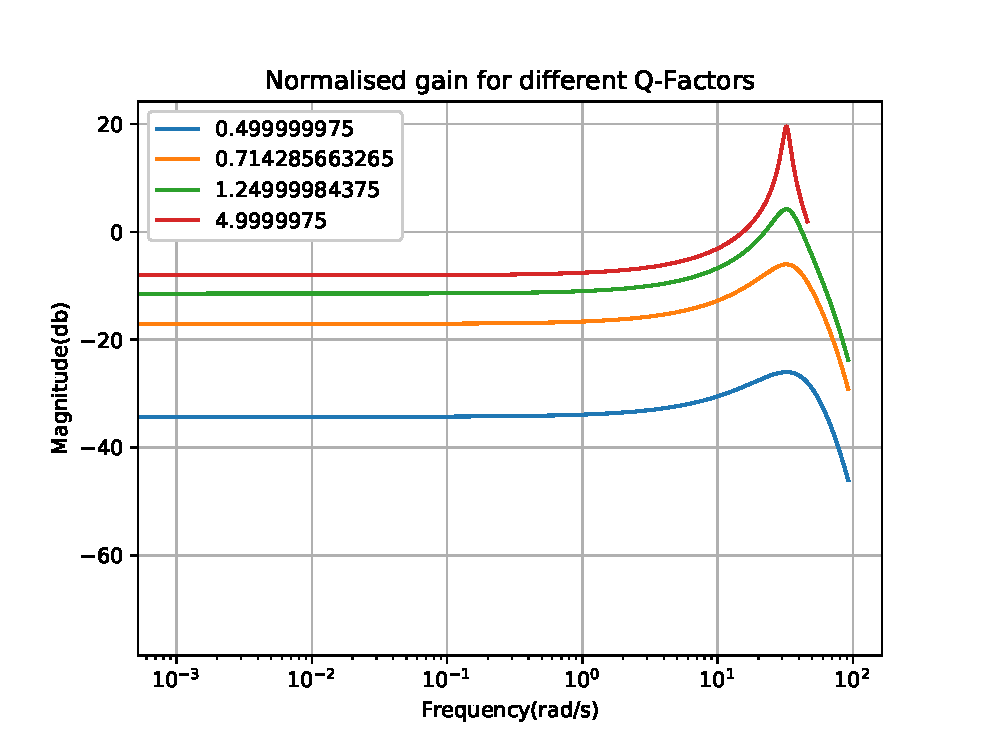
\includegraphics[width=\columnwidth]{./figs/ee18btech11030/ee18btech11030_fc.eps}
\caption{}
\label{fig:ee18btech11030_fig3} 
\end{figure}

The following is code for the plot
\begin{lstlisting}
codes/ee18btech11030/ee18btech11030.py
\end{lstlisting}
From Figure:\ref{fig:ee18btech11030_fig3} ,
\begin{itemize}
\item It is observed that maximally flat response is obtained when Q = 0.71
\item It will be seen that response of the feedback amplifier under consideration shows almost no peaking for Q$\leq$ 0.71 
\end{itemize}
\item Sketch a Pole-Zero Plot to Eq:\ref{eq:ee18btech11030_5} for a varying K

\solution :
\begin{figure}[!ht]
\centering
  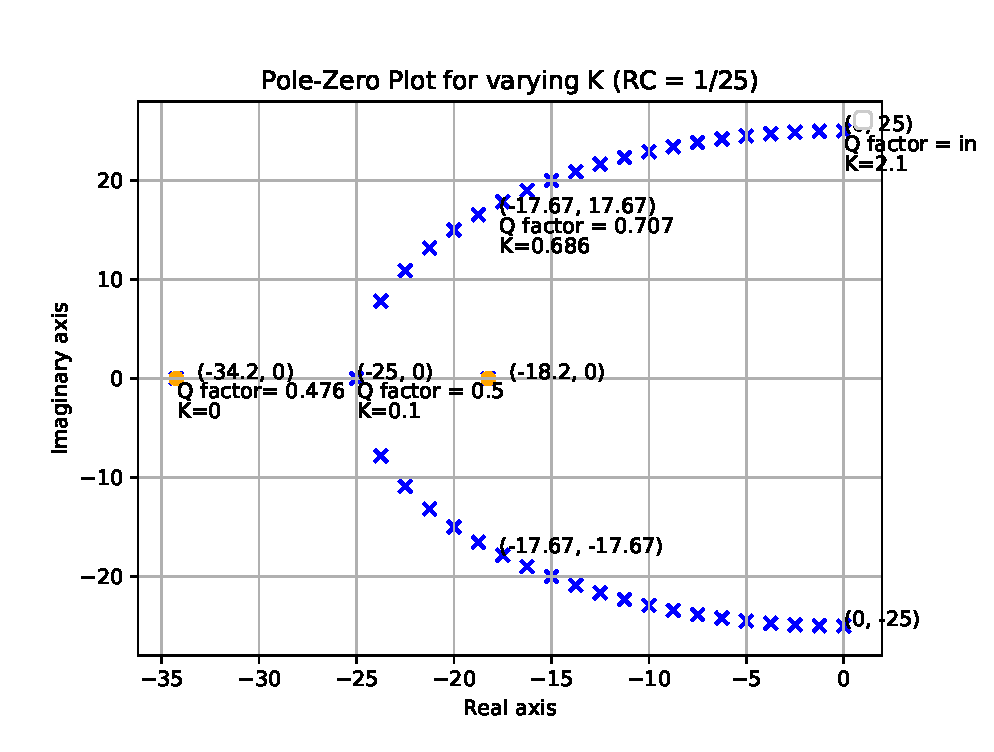
\includegraphics[width=\columnwidth]{./figs/ee18btech11030/ee18btech11030_fc1.eps}
\caption{}
\label{fig:ee18btech11030_fig4} 
\end{figure}

The following is code for the  plot
\begin{lstlisting}
codes/ee18btech11030/ee18btech11030_1.py
\end{lstlisting}
From Figure : \ref{fig:ee18btech11030_fig4} 
\begin{itemize}
\item For K = 0,the poles have Q = 0.476 and therefore located on negative real axis. 
\item As K increases poles are brought closer together and eventually coincide at K = 0.1 and Q = 0.5
\item Further increase in K results in poles becoming complex conjugate 
\item Maximally flat response is obtained when Q = 0.707,which results when K = 0.686.In this case poles are at 45\degree .
\item Oscillating response is obtained when poles are completely imaginary when Q = inf which results when K = 2.1 
\end{itemize}

\begin{table}[!ht]
\centering
 
\usetikzlibrary{decorations.markings}
\begin{circuitikz}
\draw (-4,-1) to[amp,t={+K}] (2.5,-1);
\draw (-4,-1) to (-4,2) to (-3,2) ;
\draw (-3,2)  to [capacitor=$C/10$](-3,0.5) to  (-3,0.5) node[ground]{};
\draw (-3,2) to (-2.3,2)to [R=$10R$] (-1.3,2)to (0,2) to [R=$R$] (0,5) node[label={}]{}  to (-4,5) ;
\draw (0,2) to(1,2) to  [capacitor=$C$](1.5,2) to (2.5,2) to (2.5,-1);
\draw (-4,5) to (-4,4.7) to [V=$V_s$] (-4,3.9) to (-4,3.5) node[ground]{} ;
\draw (2.5,-1) to[short, -o] (3,-1) node[label={above:$V_{out}$}]{};
\end{circuitikz}
\caption{}
\label{table:ee18btech11030_table}
\end{table}

\item Building gain K in spice simulation for circuit Fig: \ref{fig:ee18btech11030_fig1}

\solution :

\begin{itemize}
\item For K greater than 1(K = 2.1),the gain block is built using LM741 op-amp.
\begin{figure}[!ht]
	\begin{center}
		\resizebox{\columnwidth/1}{!}{\usetikzlibrary{decorations.markings}
\begin{circuitikz}
\draw (2,2)  node[op amp] (OA) {};
\draw (OA.+) -- (0,1.5) to (0,0) node[label={below:$V_i$}]{};
\draw (OA.-) -- (0,2.5) node[label={}]{} to[R,l_=$R_1$] (-2,2.5) node[ground](GND){};
\draw (OA.out) -- (3,2) node[label={}]{};
\draw (3,2) -- (4.5,2) node[label={above:$V_{o}$}]{};
\draw (3,2) -- (3,4.5) to[R=$R_2$] (0,4.5) -- (0,2.5);
\end{circuitikz}}
	\end{center}
	\caption{LM741 op-amp}
	\label{fig:ee18btech11030_fig5}
\end{figure}
\begin{align}
K = 1 + \frac{R_2}{R_1}
\implies \frac{R_2}{R_1} = 1.1
\end{align}
\item For K less than 1, the gain block is built using voltage divider circuit.
\begin{figure}[!ht]
	\begin{center}
		\resizebox{\columnwidth/1}{!}{\usetikzlibrary{decorations.markings}
\begin{circuitikz}
\ctikzset{tripoles/mos style/arrows}
\draw (1,2) to[short, -o] (0,2) node[label={above:$V_i$}]{};
\draw (1,2) to[R=$R_1$] (2,2) -- (3,2) to[R=$R_2$] (3,0) node[ground](GND){};
\draw (3,2) to[short, -o] (4,2) node[label={above:$V_o$}]{};
\end{circuitikz}}
	\end{center}
	\caption{Voltage Divider}
	\label{fig:ee18btech11030_fig6}
\end{figure}
\begin{align}
K = \frac{R_2}{R_1+R_2}
\end{align}
\end{itemize}

\item Verify the response in time domain using parameters in Table : \ref{table:ee18btech11030_table1} for K = 2.13

\solution :
\begin{figure}[!ht]
\centering
  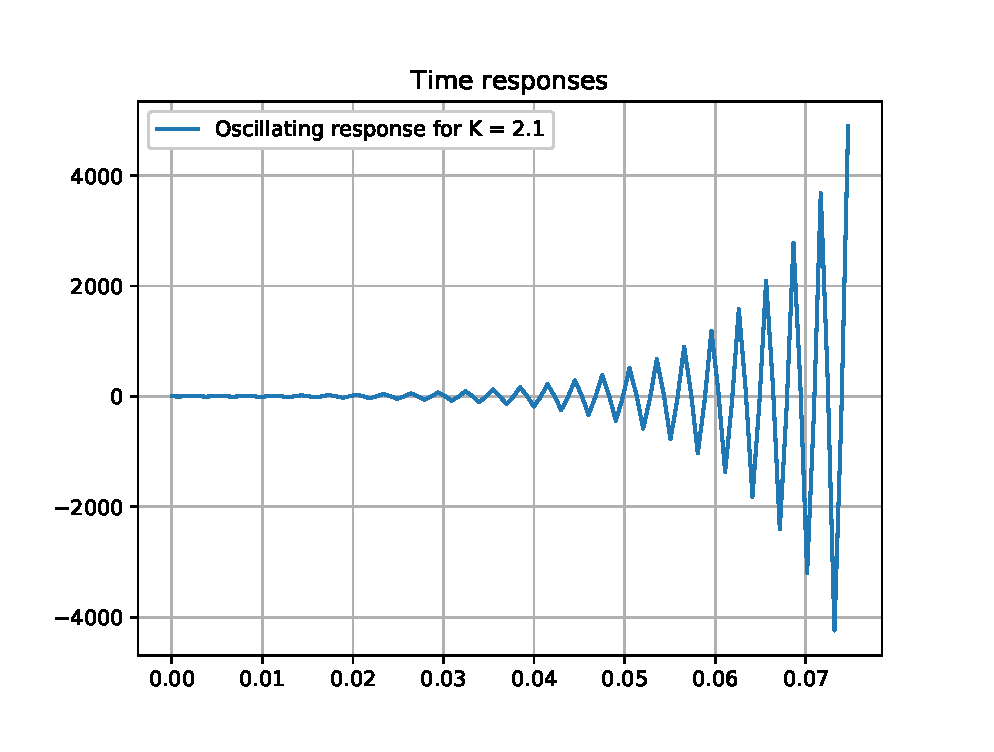
\includegraphics[width=\columnwidth]{./figs/ee18btech11030/ee18btech11030_fc2.eps}
\caption{}
\label{fig:ee18btech11030_fig7} 
\end{figure}

The following is code for the plot
\begin{lstlisting}
codes/ee18btech11030/ee18btech11030_2.py
\end{lstlisting}

\item Choose the appropriate values of R and C to simulate the circuit for K = 2.1

\solution:
\begin{table}[!ht]
\centering
%%%%%%%%%%%%%%%%%%%%%%%%%%%%%%%%%%%%%%%%%%%%%%%%%%%%%%%%%%%%%%%%%%%%%%
%%                                                                  %%
%%  This is the header of a LaTeX2e file exported from Gnumeric.    %%
%%                                                                  %%
%%  This file can be compiled as it stands or included in another   %%
%%  LaTeX document. The table is based on the longtable package so  %%
%%  the longtable options (headers, footers...) can be set in the   %%
%%  preamble section below (see PRAMBLE).                           %%
%%                                                                  %%
%%  To include the file in another, the following two lines must be %%
%%  in the including file:                                          %%
%%        \def\inputGnumericTable{}                                 %%
%%  at the beginning of the file and:                               %%
%%        \input{name-of-this-file.tex}                             %%
%%  where the table is to be placed. Note also that the including   %%
%%  file must use the following packages for the table to be        %%
%%  rendered correctly:                                             %%
%%    \usepackage[latin1]{inputenc}                                 %%
%%    \usepackage{color}                                            %%
%%    \usepackage{array}                                            %%
%%    \usepackage{longtable}                                        %%
%%    \usepackage{calc}                                             %%
%%    \usepackage{multirow}                                         %%
%%    \usepackage{hhline}                                           %%
%%    \usepackage{ifthen}                                           %%
%%  optionally (for landscape tables embedded in another document): %%
%%    \usepackage{lscape}                                           %%
%%                                                                  %%
%%%%%%%%%%%%%%%%%%%%%%%%%%%%%%%%%%%%%%%%%%%%%%%%%%%%%%%%%%%%%%%%%%%%%%



%%  This section checks if we are begin input into another file or  %%
%%  the file will be compiled alone. First use a macro taken from   %%
%%  the TeXbook ex 7.7 (suggestion of Han-Wen Nienhuys).            %%
\def\ifundefined#1{\expandafter\ifx\csname#1\endcsname\relax}


%%  Check for the \def token for inputed files. If it is not        %%
%%  defined, the file will be processed as a standalone and the     %%
%%  preamble will be used.                                          %%
\ifundefined{inputGnumericTable}

%%  We must be able to close or not the document at the end.        %%
	\def\gnumericTableEnd{\end{document}}


%%%%%%%%%%%%%%%%%%%%%%%%%%%%%%%%%%%%%%%%%%%%%%%%%%%%%%%%%%%%%%%%%%%%%%
%%                                                                  %%
%%  This is the PREAMBLE. Change these values to get the right      %%
%%  paper size and other niceties.                                  %%
%%                                                                  %%
%%%%%%%%%%%%%%%%%%%%%%%%%%%%%%%%%%%%%%%%%%%%%%%%%%%%%%%%%%%%%%%%%%%%%%

	\documentclass[12pt%
			  %,landscape%
                    ]{report}
       \usepackage[latin1]{inputenc}
       \usepackage{fullpage}
       \usepackage{color}
       \usepackage{array}
       \usepackage{longtable}
       \usepackage{calc}
       \usepackage{multirow}
       \usepackage{hhline}
       \usepackage{ifthen}



%%  End of the preamble for the standalone. The next section is for %%
%%  documents which are included into other LaTeX2e files.          %%
\else

%%  We are not a stand alone document. For a regular table, we will %%
%%  have no preamble and only define the closing to mean nothing.   %%
    \def\gnumericTableEnd{}

%%  If we want landscape mode in an embedded document, comment out  %%
%%  the line above and uncomment the two below. The table will      %%
%%  begin on a new page and run in landscape mode.                  %%
%       \def\gnumericTableEnd{\end{landscape}}
%       \begin{landscape}


%%  End of the else clause for this file being \input.              %%
\fi

%%%%%%%%%%%%%%%%%%%%%%%%%%%%%%%%%%%%%%%%%%%%%%%%%%%%%%%%%%%%%%%%%%%%%%
%%                                                                  %%
%%  The rest is the gnumeric table, except for the closing          %%
%%  statement. Changes below will alter the table's appearance.     %%
%%                                                                  %%
%%%%%%%%%%%%%%%%%%%%%%%%%%%%%%%%%%%%%%%%%%%%%%%%%%%%%%%%%%%%%%%%%%%%%%

\providecommand{\gnumericmathit}[1]{#1} 
%%  Uncomment the next line if you would like your numbers to be in %%
%%  italics if they are italizised in the gnumeric table.           %%
%\renewcommand{\gnumericmathit}[1]{\mathit{#1}}
\providecommand{\gnumericPB}[1]%
{\let\gnumericTemp=\\#1\let\\=\gnumericTemp\hspace{0pt}}
 \ifundefined{gnumericTableWidthDefined}
        \newlength{\gnumericTableWidth}
        \newlength{\gnumericTableWidthComplete}
        \newlength{\gnumericMultiRowLength}
        \global\def\gnumericTableWidthDefined{}
 \fi
%% The following setting protects this code from babel shorthands.  %%
 \ifthenelse{\isundefined{\languageshorthands}}{}{\languageshorthands{english}}
%%  The default table format retains the relative column widths of  %%
%%  gnumeric. They can easily be changed to c, r or l. In that case %%
%%  you may want to comment out the next line and uncomment the one %%
%%  thereafter                                                      %%
\providecommand\gnumbox{\makebox[0pt]}
%%\providecommand\gnumbox[1][]{\makebox}

%% to adjust positions in multirow situations                       %%
\setlength{\bigstrutjot}{\jot}
\setlength{\extrarowheight}{\doublerulesep}

%%  The \setlongtables command keeps column widths the same across  %%
%%  pages. Simply comment out next line for varying column widths.  %%
\setlongtables

\setlength\gnumericTableWidth{%
	50pt+%
	65pt+%
0pt}
\def\gumericNumCols{2}
\setlength\gnumericTableWidthComplete{\gnumericTableWidth+%
         \tabcolsep*\gumericNumCols*2+\arrayrulewidth*\gumericNumCols}
\ifthenelse{\lengthtest{\gnumericTableWidthComplete > \linewidth}}%
         {\def\gnumericScale{\ratio{\linewidth-%
                        \tabcolsep*\gumericNumCols*2-%
                        \arrayrulewidth*\gumericNumCols}%
{\gnumericTableWidth}}}%
{\def\gnumericScale{1}}

%%%%%%%%%%%%%%%%%%%%%%%%%%%%%%%%%%%%%%%%%%%%%%%%%%%%%%%%%%%%%%%%%%%%%%
%%                                                                  %%
%% The following are the widths of the various columns. We are      %%
%% defining them here because then they are easier to change.       %%
%% Depending on the cell formats we may use them more than once.    %%
%%                                                                  %%
%%%%%%%%%%%%%%%%%%%%%%%%%%%%%%%%%%%%%%%%%%%%%%%%%%%%%%%%%%%%%%%%%%%%%%

\ifthenelse{\isundefined{\gnumericColA}}{\newlength{\gnumericColA}}{}\settowidth{\gnumericColA}{\begin{tabular}{@{}p{53pt*\gnumericScale}@{}}x\end{tabular}}
\ifthenelse{\isundefined{\gnumericColB}}{\newlength{\gnumericColB}}{}\settowidth{\gnumericColB}{\begin{tabular}{@{}p{93pt*\gnumericScale}@{}}x\end{tabular}}

\begin{tabular}[c]{%
	b{\gnumericColA}%
	b{\gnumericColB}%
	}

%%%%%%%%%%%%%%%%%%%%%%%%%%%%%%%%%%%%%%%%%%%%%%%%%%%%%%%%%%%%%%%%%%%%%%
%%  The longtable options. (Caption, headers... see Goosens, p.124) %%
%	\caption{The Table Caption.}             \\	%
% \hline	% Across the top of the table.
%%  The rest of these options are table rows which are placed on    %%
%%  the first, last or every page. Use \multicolumn if you want.    %%

%%  Header for the first page.                                      %%
%	\multicolumn{2}{c}{The First Header} \\ \hline 
%	\multicolumn{1}{c}{colTag}	%Column 1
%	&\multicolumn{1}{c}{colTag}	\\ \hline %Last column
%	\endfirsthead

%%  The running header definition.                                  %%
%	\hline
%	\multicolumn{2}{l}{\ldots\small\slshape continued} \\ \hline
%	\multicolumn{1}{c}{colTag}	%Column 1
%	&\multicolumn{1}{c}{colTag}	\\ \hline %Last column
%	\endhead

%%  The running footer definition.                                  %%
%	\hline
%	\multicolumn{2}{r}{\small\slshape continued\ldots} \\
%	\endfoot

%%  The ending footer definition.                                   %%
%	\multicolumn{2}{c}{That's all folks} \\ \hline 
%	\endlastfoot
%%%%%%%%%%%%%%%%%%%%%%%%%%%%%%%%%%%%%%%%%%%%%%%%%%%%%%%%%%%%%%%%%%%%%%

\hhline{|-|-}
	 \multicolumn{1}{|p{\gnumericColA}|}%
	{\gnumericPB{\centering}\gnumbox{\textbf{Parameter}}}
	&\multicolumn{1}{p{\gnumericColB}|}%
	{\gnumericPB{\centering}\gnumbox{\textbf{Value}}}
\\
\hhline{|--|}
	 \multicolumn{1}{|p{\gnumericColA}|}%
	{\gnumericPB{\raggedright}\gnumbox[l]{$R_{1}$}}
	&\multicolumn{1}{p{\gnumericColB}|}%
	{\gnumericPB{\raggedright}\gnumbox[l]{$10k\Omega$}}
\\
\hhline{|--|}
	 \multicolumn{1}{|p{\gnumericColA}|}%
	{\gnumericPB{\raggedright}\gnumbox[l]{$R_{2}$}}
	&\multicolumn{1}{p{\gnumericColB}|}%
	{\gnumericPB{\raggedright}\gnumbox[l]{$11.3k\Omega$}}
\\
\hhline{|--|}
	 \multicolumn{1}{|p{\gnumericColA}|}%
	{\gnumericPB{\raggedright}\gnumbox[l]{$R$}}
	&\multicolumn{1}{p{\gnumericColB}|}%
	{\gnumericPB{\raggedright}\gnumbox[l]{$10k\Omega$}}
\\
\hhline{|--|}
	 \multicolumn{1}{|p{\gnumericColA}|}%
	{\gnumericPB{\raggedright}\gnumbox[l]{$10R$}}
	&\multicolumn{1}{p{\gnumericColB}|}%
	{\gnumericPB{\raggedright}\gnumbox[l]{$100k\Omega$}}
\\
\hhline{|--|}
	 \multicolumn{1}{|p{\gnumericColA}|}%
	{\gnumericPB{\raggedright}\gnumbox[l]{$C/10$}}
	&\multicolumn{1}{p{\gnumericColB}|}%
	{\gnumericPB{\raggedright}\gnumbox[l]{$1.6nF$}}
\\

\hhline{|--|}
	 \multicolumn{1}{|p{\gnumericColA}|}%
	{\gnumericPB{\raggedright}\gnumbox[l]{$C$}}
	&\multicolumn{1}{p{\gnumericColB}|}%
	{\gnumericPB{\raggedright}\gnumbox[l]{$16nF$}}

\\
\hhline{|-|-|}
\end{tabular}

\ifthenelse{\isundefined{\languageshorthands}}{}{\languageshorthands{\languagename}}
\gnumericTableEnd

\caption{}
\label{table:ee18btech11030_table1}
\end{table}
\item Verify the response using the spice model

\solution :

\begin{itemize}
    \item Figure \ref{fig:ee18btech11030_fig8} is the spice simulated output for K = 2.1 using Table \ref{table:ee18btech11030_table1} parameters.
    \item The following is the netlist for simulated circuit.
\begin{lstlisting}
spice/ee18btech11030/ee18btech11030.net
\end{lstlisting}
    \item The following is code for generating output
\begin{lstlisting}
spice/ee18btech11030/ee18btech11030.py
\end{lstlisting}
    
\end{itemize}
\begin{figure}[!ht]
\centering
  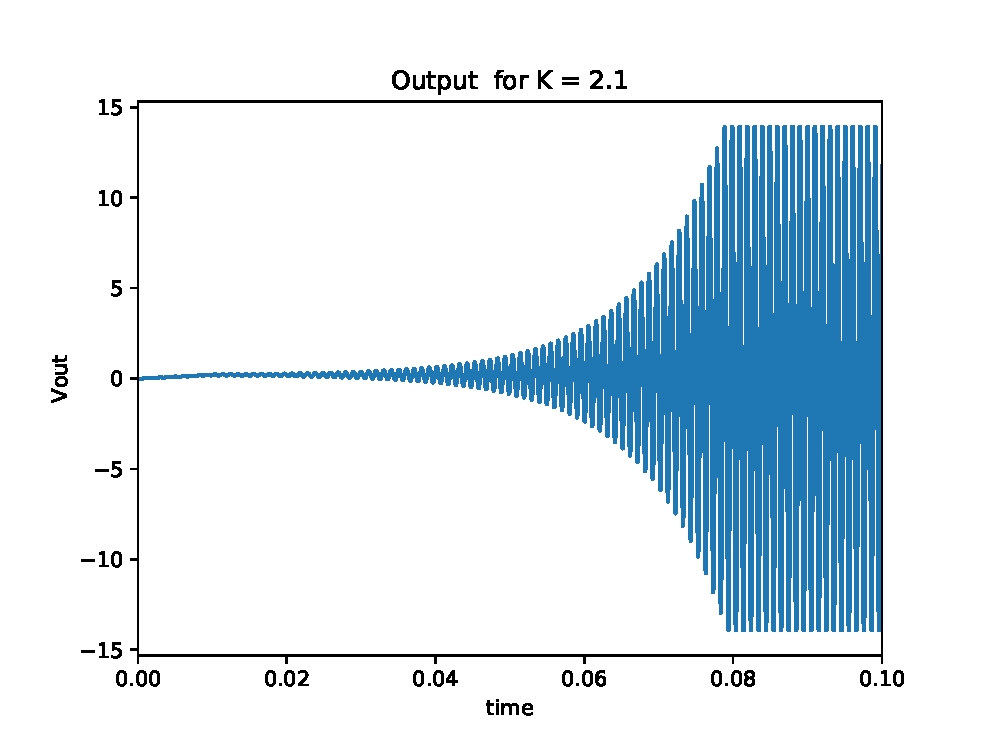
\includegraphics[width=\columnwidth]{./figs/ee18btech11030/ee18btech11030_spice_fc3.eps}
\caption{}
\label{fig:ee18btech11030_fig8} 
\end{figure}

\item Choose the appropriate values of R and C to simulate the circuit for K = 0.1 and K = 0.686

\solution :

\begin{table}[!ht]
\centering
\usetikzlibrary{decorations.markings}
\begin{circuitikz}
\ctikzset{tripoles/mos style/arrows}
\draw (1,2) to[short, -o] (0,2) node[label={above:$V_i$}]{};
\draw (1,2) to[R=$R_1$] (2,2) -- (3,2) to[R=$R_2$] (3,0) node[ground](GND){};
\draw (3,2) to[short, -o] (4,2) node[label={above:$V_o$}]{};
\end{circuitikz}
\caption{}
\label{table:ee18btech11030_table2}
\end{table}
\item Verify the response using the spice model

\solution 

\begin{figure}[!ht]
\centering
  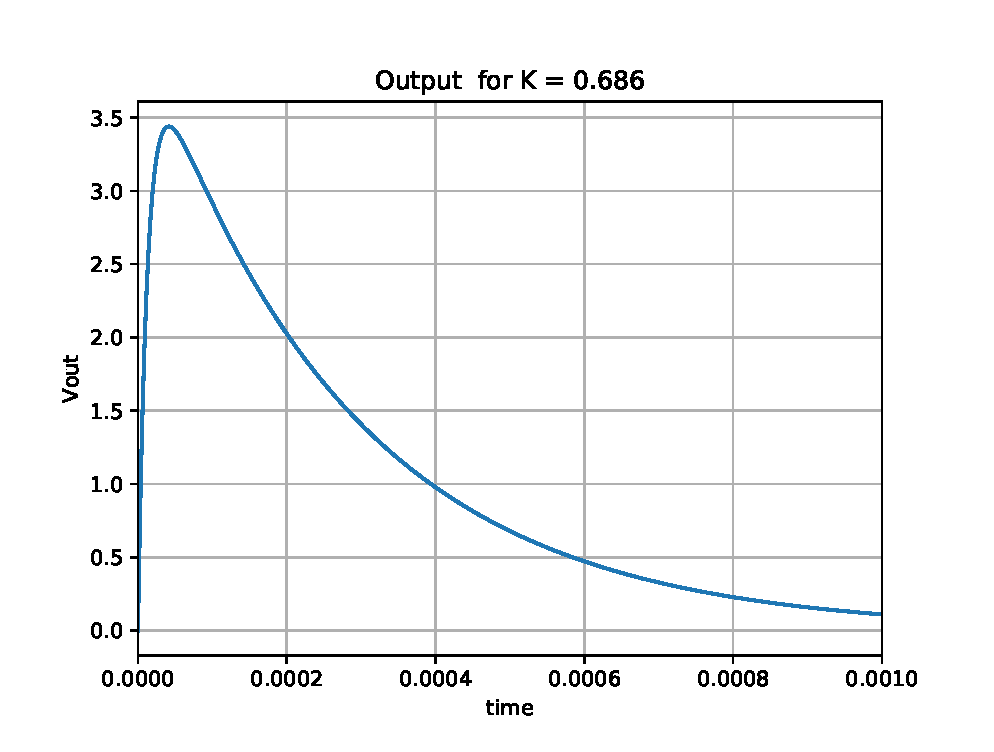
\includegraphics[width=\columnwidth]{./figs/ee18btech11030/ee18btech11030_spice_fc4.eps}
\caption{}
\label{fig:ee18btech11030_fig9} 
\end{figure}

\begin{itemize}
    \item Figure \ref{fig:ee18btech11030_fig9} is the spice simulated output for K = 0.686 using Table \ref{table:ee18btech11030_table2} parameters.
    \item The following is the netlist for simulated circuit.
\begin{lstlisting}
spice/ee18btech11030/ee18btech11030_1.net
\end{lstlisting}
    \item The following is code for generating output
\begin{lstlisting}
spice/ee18btech11030/ee18btech11030_1.py
\end{lstlisting}
\end{itemize}
\begin{figure}[!ht]
\centering
  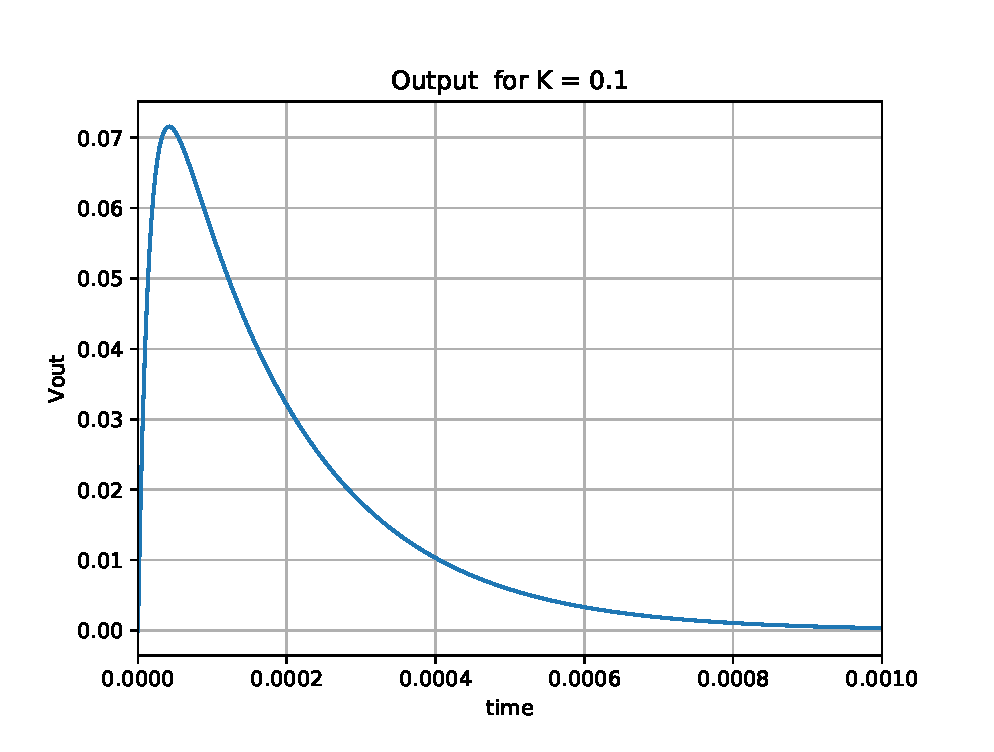
\includegraphics[width=\columnwidth]{./figs/ee18btech11030/ee18btech11030_spice_fc5.eps}
\caption{}
\label{fig:ee18btech11030_fig10} 
\end{figure}
\begin{itemize}
    \item Figure \ref{fig:ee18btech11030_fig10} is the spice simulated output for K = 0.1 using Table \ref{table:ee18btech11030_table2} parameters.
    \item The following is the netlist for simulated circuit.
\begin{lstlisting}
spice/ee18btech11030/ee18btech11030_2.net
\end{lstlisting}
    \item The following is code for generating output
\begin{lstlisting}
spice/ee18btech11030/ee18btech11030_2.py
\end{lstlisting}
\end{itemize}
\end{enumerate}
